\chapter{Kombinatoriikka}

Kombinatoriikka tarkoittaa yhdistelmien määrän laskemista.
Tavoitteena on yleensä laskea yhdistelmät
tehokkaasti niin, että jokaista yhdistelmää
ei tarvitse muodostaa erikseen, vaan yhteismäärän
saa selville tehokkaammin hyödyntämällä säännöllisyyksiä ja
dynaamista ohjelmointia.

\section{Perustekniikat}

\subsubsection*{Yhdistelmät}

Jos yhdistelmä muodostuu $n$ osasta ja jokainen osa
voidaan valita $k$ tavalla, yhdistelmiä on yhteensä $k^n$.
Esimerkiksi $n$-pituisia bittijonoja on $2^n$,
koska jokainen jonon bitti voidaan valita 2 tavalla.

Yleisemmin jos yhdistelmä muodostuu $n$ osasta,
joista osan 1 voi valita $k_1$ tavalla,
osan 2 voi valita $k_2$ tavalla, jne.,
yhdistelmien määrä on $k_1 \cdot k_2 \cdots k_n$.

\subsubsection*{Permutaatiot}

Permutaatio tarkoittaa joukon alkioiden järjestystä.
Jos joukossa on $n$ alkiota,
niin siitä voi muodostaa $n!$ permutaatiota,
koska ensimmäinen alkio voidaan valita $n$ tavalla,
toinen $(n-1)$ tavalla, jne.
Esimerkiksi kirjaimet \texttt{ABC} voidaan järjestää
6 tavalla:
\texttt{ABC}, \texttt{ACB}, \texttt{BAC}, \texttt{BCA},
\texttt{CAB} ja \texttt{CBA}.

\subsubsection*{Rekursiokaava}

Kombinatorisen tehtävän ratkaisun pystyy usein ilmaisemaan
rekursiolla, jolloin vastauksen saa laskettua tehokkaasti
dynaamisella ohjelmoinnilla.
Näin on esimerkiksi seuraavassa tehtävässä:

\begin{task}
Tehtäväsi on laskea, monessako $n$ bitin jonossa
ei ole vierekkäin kahta ykkösbittiä.
Esimerkiksi jos $n=4$, vastaus on 8,
koska bittijonot ovat \texttt{0000}, \texttt{0001},
\texttt{0010}, \texttt{0100}, \texttt{0101},
\texttt{1000}, \texttt{1001} ja \texttt{1010}.
\end{task}

Vastaus selviää funktiolla $f(n,k)$,
jossa $n$ on bittijonon pituus ja $k$ on viimeinen bitti (0 tai 1).
Tätä funktiota käyttäen $n$ bitin jonojen määrä
on summa $f(n,0)+f(n,1)$.
Rekursiivinen kaava on seuraava:

\begin{equation*}
    f(n,k) = \begin{cases}
               1               & n = 1\\
               f(n-1,0)+f(n-1,1) & k = 0\\
               f(n-1,0) & k = 1\\
           \end{cases}
\end{equation*}

Kaavan ideana on, että jos viimeinen bitti on 0,
sitä ennen voi olla sekä bitti 0 että bitti 1,
ja jos viimeinen bitti on 1, sitä ennen on
pakko olla bitti 0.


\section{Binomikerroin}

Binomikerroin ${n \choose k}$ ilmaisee, montako
erilaista $k$ alkion osajoukkoa $n$ alkion joukosta
voidaan muodostaa.
Esimerkiksi ${5 \choose 2}=10$,
koska joukosta $\{A,B,C,D,E\}$
voidaan muodostaa 10 erilaista 2 alkion osajoukkoa:
\[ \{A,B\}, \{A,C\}, \{A,D\}, \{A,E\}, \{B,C\}, 
\{B,D\}, \{B,E\}, \{C,D\}, \{C,E\}, \{D,E\} \]

\subsubsection*{Laskutapa 1}

Tavallisin tapa laskea binomikerroin on
käyttää kaavaa
\[ {n \choose k}  = \frac{n!}{k!(n-k)!} .\]
Esimerkiksi
\[ {5 \choose 2} = \frac{5!}{2!3!} = \frac{120}{12} = 10. \]
Huomaa myös, että
\[ {n \choose k} = {n \choose n-k},\]
koska $k$ alkion valinta osajoukkoon tarkoittaa
samalla $n-k$ alkion valintaa osajoukon ulkopuolelle.

\subsubsection*{Laskutapa 2}

Binomikertoimen voi myös laskea rekursiivisesti kaavalla

\[  {n \choose k} = {n-1 \choose k-1} + {n-1 \choose k}.  \]

Pohjatapauksina ${n \choose 0} = 1$,
koska tyhjän osajoukon voi muodostaa aina tasan yhdellä tavalla,
ja ${n \choose k} = 0$, jos $k>n$,
koska $n$ alkiosta ei ole mahdollista valita
yli $n$ alkion osajoukkoa.

Rekursion voi perustella tarkastelemalla yksittäistä
joukon alkiota $x$. Jos alkio $x$ valitaan osajoukkoon,
täytyy vielä valita $n-1$ alkiosta $k-1$ alkiota.
Jos taas alkiota $x$ ei valita,
täytyy vielä valita $n-1$ alkiosta $k$ alkiota.

\subsubsection*{Multinomikerroin}

Binomikertoimen yleistys on multinomikerroin

\[ {n \choose k_1,k_2,\ldots,k_m} = \frac{n!}{k_1! k_2! \cdots k_m!}, \]

missä $k_1+k_2+\cdots+k_m=n$.
Multinomikerroin ilmaisee, monellako tavalla $n$ alkiota voidaan jakaa osajoukkoihin,
joiden koot ovat $k_1,k_2,\ldots,k_m$.
Jos $m=2$, niin multinomikertoimen kaava vastaa binomikertoimen kaavaa.

\subsubsection*{Hatut ja pallot}

Binomikertoimen avulla voi ratkaista myös seuraavan tehtävän:

\begin{task}
Rivissä on $n$ hattua, joihin sijoitetaan $m$ palloa.
Montako erilaista tapaa tähän on?
Esimerkiksi jos $n=3$ ja $m=2$, niin tapoja on 6:
$[0,0,2]$, $[0,1,1]$, $[0,2,0]$, $[1,0,1]$, $[1,1,0]$,
$[2,0,0]$.
\end{task}

\noindent
Ratkaisu tehtävään on ${n+m-1 \choose m}$.
Jokaisen sijoitustavan voi ilmaista merkkijonona, jossa \texttt{o}
kuvaa palloa ja \texttt{|} on kahden hatun raja.
Merkkijonon pituus on $n+m-1$, koska palloja on $m$
ja hatun rajoja on $n-1$,
ja siitä valitaan $m$ paikkaa palloille.
Esimerkiksi sijoitustapaa $[1,0,1]$
vastaa merkkijono \texttt{o||o}.

\section{Muita funktioita}

\subsubsection*{Catalanin luvut}

Catalanin luku $C_n$ ilmaisee,
montako tapaa on muodostaa kelvollinen sulkulauseke
$n$ alkusulusta ja $n$ loppusulusta.
Esimerkiksi $C_3=5$, koska vastaavat sulkulausekkeet
ovat \texttt{()()()}, \texttt{(())()},
\texttt{()(())}, \texttt{((()))} ja \texttt{(()())}.

Luonteva tapa laskea Catalanin lukuja
on käyttää rekursiokaavaa

\[ C_n = \sum_{i=0}^{n-1} C_i C_{n-i-1}, \]

jossa pohjatapauksena on $C_0=1$.
Catalanin luvut saa laskettua myös binomikertoimen avulla kaavalla

\[ C_n = \frac{1}{n+1} {2n \choose n}. \]

\subsubsection*{Stirlingin luvut}

Stirlingin luku ${n \brace k}$ ilmaisee,
montako tapaa on jakaa $n$ alkion joukko
$k$ epätyhjäksi osajoukoksi.
Esimerkiksi ${4 \brace 2}=7$, koska
joukon $\{A,B,C,D\}$ jakotavat 2
epätyhjäksi osajoukoksi ovat
 $\{A,B,C\}$ ja $\{D\}$, 
 $\{A,B,D\}$ ja $\{C\}$,
 $\{A,C,D\}$ ja $\{B\}$,
 $\{B,C,D\}$ ja $\{A\}$,
  $\{A,B\}$ ja $\{C,D\}$,
  $\{A,C\}$ ja $\{B,D\}$, sekä
  $\{A,D\}$ ja $\{B,C\}$.

\noindent
Stirlingin lukuja voi laskea rekursiivisesti kaavalla
\[ {n \brace k} = k{n-1 \brace k} + {n-1 \brace k-1}, \]
jossa pohjatapauksina ${n \brace k}=0$,
kun $k=0$ tai $k>n$, ja ${n \brace k}=1$, kun $k=1$.

\section{Sisään-ulos-periaate}

Sisään-ulos-periaate eli inkluusio-ekskluusio
on tekniikka, jonka avulla pystyy laskemaan
joukkojen yhdisteen koon leikkausten
kokojen perusteella ja päinvastoin.
Yksinkertainen esimerkki periaatteesta on kaava
\[ |A \cup B| = |A| + |B| - |A \cap B|,\]
jossa $A$ ja $B$ ovat joukkoja ja $|X|$ on joukon koko.
Seuraava kuva havainnollistaa kaavaa,
kun joukot ovat tason ympyröitä:

\begin{center}
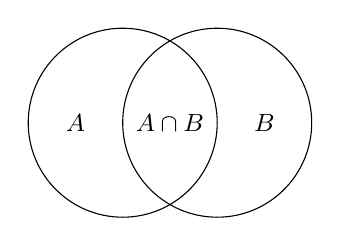
\begin{tikzpicture}[scale=0.8]

\draw (0,0) circle (1.5);
\draw (1.5,0) circle (1.5);

\node at (-0.75,0) {\small $A$};
\node at (2.25,0) {\small $B$};
\node at (0.75,0) {\small $A \cap B$};

\end{tikzpicture}
\end{center}

Tavoitteena on laskea, kuinka suuri on yhdiste $A \cup B$
eli alue, joka on ainakin toisen ympyrän sisällä.
Kuvan mukaisesti yhdisteen $A \cup B$ koko
saadaan laskemalla ensin yhteen ympyröiden $A$ ja $B$ koot
ja vähentämällä siitä sitten leikkauksen $A \cap B$ koko.

Samaa ideaa voi soveltaa, kun joukkoja on enemmän.
Kolmen joukon tapauksessa kaavasta tulee
\[ |A \cup B \cup C| = |A| + |B| + |C| - |A \cap B|  - |A \cap C|  - |B \cap C| + |A \cap B \cap C| \]
ja vastaava kuva on


\begin{center}
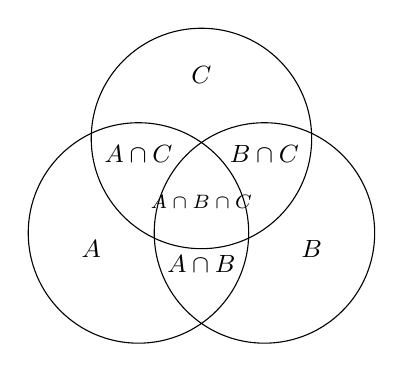
\begin{tikzpicture}[scale=0.8]

\draw (0,0) circle (1.75);
\draw (2,0) circle (1.75);
\draw (1,1.5) circle (1.75);

\node at (-0.75,-0.25) {\small $A$};
\node at (2.75,-0.25) {\small $B$};
\node at (1,2.5) {\small $C$};
\node at (1,-0.5) {\small $A \cap B$};
\node at (0,1.25) {\small $A \cap C$};
\node at (2,1.25) {\small $B \cap C$};
\node at (1,0.5) {\scriptsize $A \cap B \cap C$};

\end{tikzpicture}
\end{center}

Yleisessä tapauksessa yhdisteen $X_1 \cup X_2 \cup \cdots \cup X_n$
koon saa laskettua käymällä läpi kaikki tavat muodostaa
leikkaus joukoista $X_1,X_2,\ldots,X_n$.
Parittoman määrän joukkoja sisältävät leikkaukset
lasketaan mukaan positiivisina ja
parillisen määrän negatiivisina.

Huomaa, että vastaavat kaavat toimivat myös käänteisesti
leikkauksen koon laskemiseen yhdisteiden kokojen perusteella.
Esimerkiksi

\[ |A \cap B| = |A| + |B| - |A \cup B|\]

ja
\[ |A \cap B \cap C| = |A| + |B| + |C| - |A \cup B|  - |A \cup C|  - |B \cup C| + |A \cup B \cup C| .\]

\subsubsection*{Esimerkki}

\begin{task}
Taulukossa on luvut $1,2,\ldots,n$ järjestyksessä.
Tehtäväsi on muuttaa järjestystä niin,
että mikään luvuista ei jää alkuperäiselle paikalleen.
Montako tapaa tähän on olemassa?
Esimerkiksi jos $n=3$, ratkaisuja on 2: $(2,3,1)$ ja $(3,1,2)$
\end{task}

Yksi tapa lähestyä tehtävää on käyttää sisään-ulos-periaatetta.
Olkoon joukko $X_k$ niiden permutaatioiden joukko,
jossa kohdassa $k$ on luku $k$.
Esimerkiksi jos $n=3$, niin joukot ovat seuraavat:
\[
\begin{array}{lcl}
X_1 & = & \{(1,2,3),(1,3,2)\} \\
X_2 & = & \{(1,2,3),(3,2,1)\} \\
X_3 & = & \{(1,2,3),(2,1,3)\} \\
\end{array}
\]
Näitä joukkoja käyttäen ratkaisujen määrä on
\[ n! - |X_1 \cup X_2 \cup \cdots \cup X_n|, \]
eli
riittää laskea joukkojen yhdisteen koko.
Tämä palautuu sisään-ulos-peri\-aatteen avulla
joukkojen leikkausten kokojen laskemiseen,
mikä onnistuu tehokkaasti.
Esimerkiksi kun $n=3$, joukon $|X_1 \cup X_2 \cup X_3|$ koko on
\[
\begin{array}{lcl}
 & & |X_1| + |X_2| + |X_3| - |X_1 \cap X_2|  - |X_1 \cap X_3|  - |X_2 \cap X_3| + |X_1 \cap X_2 \cap X_3| \\
 & = & 2+2+2-1-1-1+1 \\
 & = & 4, \\
\end{array}
\]
joten ratkaisujen määrä on $3!-4=2$.

\section{Burnsiden lemma}

Burnsiden lemma laskee yhdistelmien määrän niin,
että symmetrisistä yhdistelmistä lasketaan
mukaan vain yksi edustaja.
Burnsiden lemman mukaan yhdistelmien määrä on
\[\sum_{k=1}^n \frac{c(k)}{n},\]
missä yhdistelmän asentoa voi muuttaa $n$ tavalla
ja $c(k)$ on niiden yhdistelmien määrä,
jotka pysyvät ennallaan, kun asentoa
muutetaan tavalla $k$.

\newpage
\noindent
Tutustumme Burnsiden lemmaan seuraavan tehtävän kautta:

\begin{task}
Helminauhassa on $n$ helmeä,
joista jokaisen väri on väliltä $1,2,\ldots,m$.
Montako erilaista helminauhaa on olemassa?
Kaksi helminauhaa ovat symmetriset,
jos ne voi saada näyttämään samalta pyörittämällä.
\end{task}

\noindent
Esimerkiksi helminauhan
\begin{center}
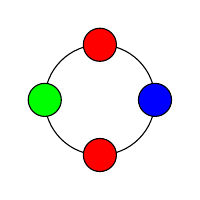
\begin{tikzpicture}[scale=0.7]
\draw[fill=white] (0,0) circle (1);
\draw[fill=red] (0,1) circle (0.3);
\draw[fill=blue] (1,0) circle (0.3);
\draw[fill=red] (0,-1) circle (0.3);
\draw[fill=green] (-1,0) circle (0.3);
\end{tikzpicture}
\end{center}
kanssa symmetriset helminauhat ovat seuraavat:
\begin{center}
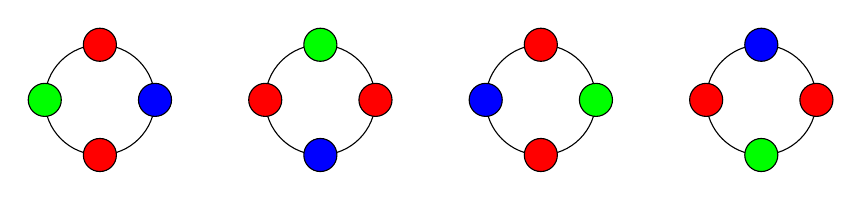
\begin{tikzpicture}[scale=0.7]
\draw[fill=white] (0,0) circle (1);
\draw[fill=red] (0,1) circle (0.3);
\draw[fill=blue] (1,0) circle (0.3);
\draw[fill=red] (0,-1) circle (0.3);
\draw[fill=green] (-1,0) circle (0.3);

\draw[fill=white] (4,0) circle (1);
\draw[fill=green] (4+0,1) circle (0.3);
\draw[fill=red] (4+1,0) circle (0.3);
\draw[fill=blue] (4+0,-1) circle (0.3);
\draw[fill=red] (4+-1,0) circle (0.3);

\draw[fill=white] (8,0) circle (1);
\draw[fill=red] (8+0,1) circle (0.3);
\draw[fill=green] (8+1,0) circle (0.3);
\draw[fill=red] (8+0,-1) circle (0.3);
\draw[fill=blue] (8+-1,0) circle (0.3);

\draw[fill=white] (12,0) circle (1);
\draw[fill=blue] (12+0,1) circle (0.3);
\draw[fill=red] (12+1,0) circle (0.3);
\draw[fill=green] (12+0,-1) circle (0.3);
\draw[fill=red] (12+-1,0) circle (0.3);
\end{tikzpicture}
\end{center}
Tapoja muuttaa asentoa on $n$,
koska helminauhaa voi pyörittää $0,1,\ldots,n-1$
askelta myötäpäivään.
Jos helminauhaa pyörittää 0 askelta,
kaikki $m^n$ väritystä säilyvät ennallaan.
Jos taas helminauhaa pyörittää 1 askeleen,
vain $m$ yksiväristä helminauhaa säilyy ennallaan.

Yleisemmin kun helminauhaa pyörittää $k$ askelta,
ennallaan säilyvien yhdistelmien määrä on
\[m^{\textrm{syt}(k,n)},\]
missä $\textrm{syt}(k,n)$ on lukujen $k$ ja $n$
suurin yhteinen tekijä.
Tämä johtuu siitä, että $\textrm{syt}(k,n)$-kokoiset
pätkät helmiä siirtyvät toistensa paikoille
$k$ askelta eteenpäin.
Niinpä helminauhojen määrä on
Burnsiden lemman mukaan
\[\sum_{i=0}^{n-1} \frac{m^{\textrm{syt}(i,n)}}{n}. \]
Esimerkiksi kun helminauhan pituus on 4
ja värejä on 3, helminauhoja on
\[\frac{3^4+3+3^2+3}{4} = 24. \]

